\documentclass{beamer}


\usetheme{default}
\usecolortheme{dolphin} 

\usepackage{booktabs} % 用于美化表格
\usepackage{array} % 允许调整列格式

\title{Weekly Report about\\
Fixed Effects, "Banking Market", and Samples}
\date{\today}

\begin{document}
\begin{frame}
  \titlepage
\end{frame}




\begin{frame}{Content}
  \tableofcontents
\end{frame}


\section{Definition of “banking market” in GP wp}

\begin{frame}
    \vfill
    \centering
    {\usebeamercolor[fg]{structure}Definition of “banking market” in GP wp}
    \vfill
\end{frame}

\begin{frame}{Definition of “banking market” in GP wp}

In P16 footnote, \textit{Regional Federal Reserve Banks define “banking markets”. The geographic delimitation of each banking market is available online: \href{https://cassidi.stlouisfed.org/index}{\usebeamercolor[fg]{structure}{https://cassidi.stlouisfed.org/index}}.}

\vspace{2em}

\begin{itemize}
    \item Each “banking market” is composed of several cities, and sometimes, one banking market is a partial county.
    \item Ratewatch data have the “city” field, so we can match “banking market” using “city”.
    \item Besides, CASSIDI also has HHI data for a specific “banking market”.
\end{itemize}

\end{frame}


\section{Adding county fixed effects}



\begin{frame}
    \vfill
    \centering
    {\usebeamercolor[fg]{structure}Adding county fixed effects}
    \vfill
\end{frame}

\begin{frame}{12MCD0K, multi-branches sample}
\begin{center}
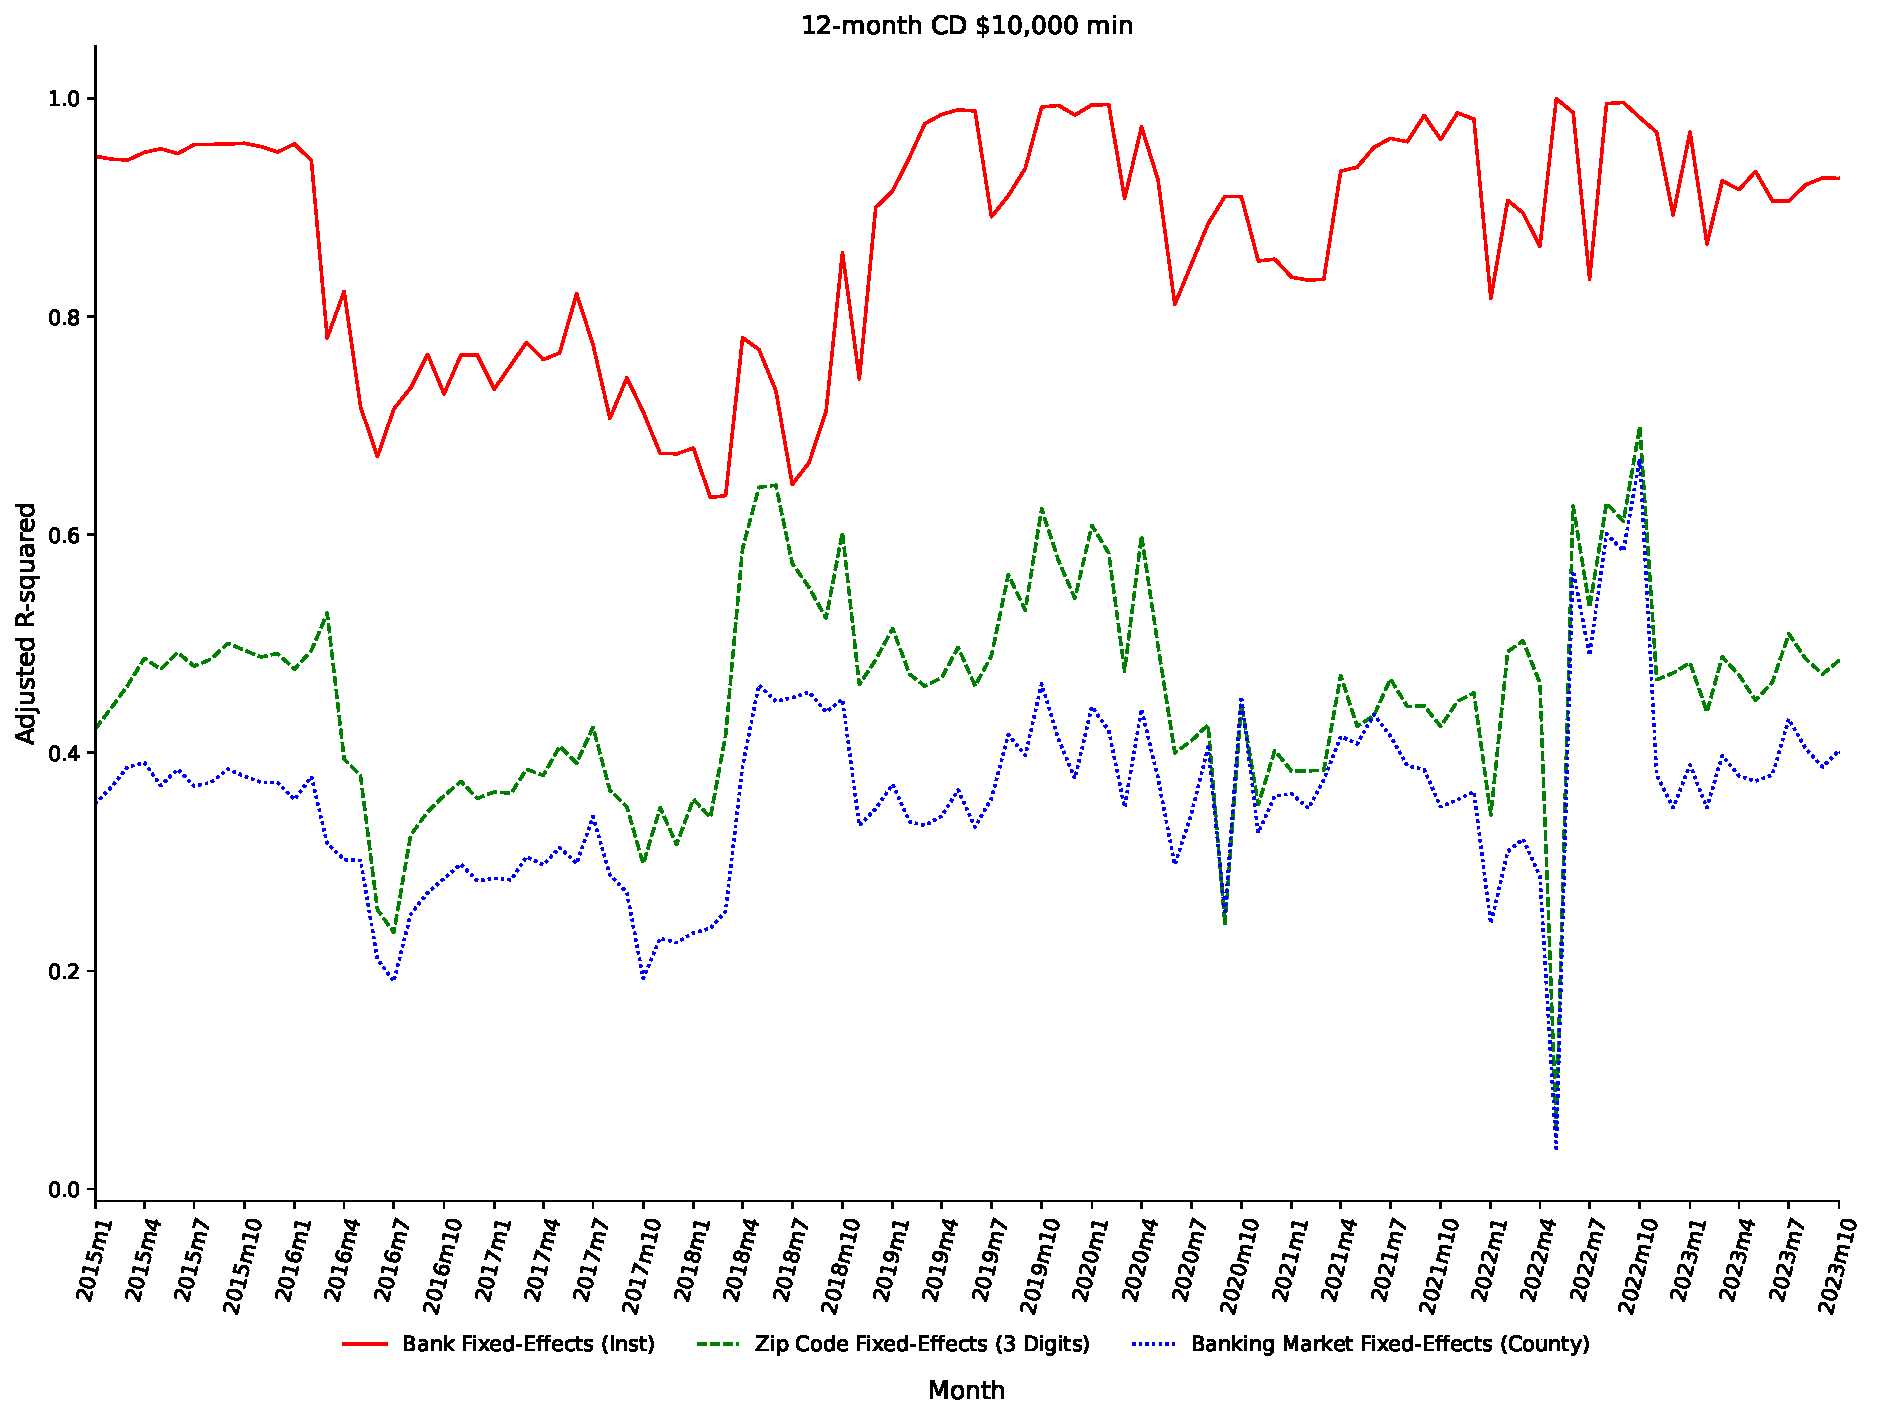
\includegraphics[width=1\textwidth]{figure/multi_branch_sample_932466/3_fixed_effects_same_as_GP_wp/12MCD10K_adjusted_R2_Rate_3_fixed_effects.pdf} 
\end{center}
\end{frame}

\begin{frame}{INTCK2.5K, multi-branches sample}
\begin{center}
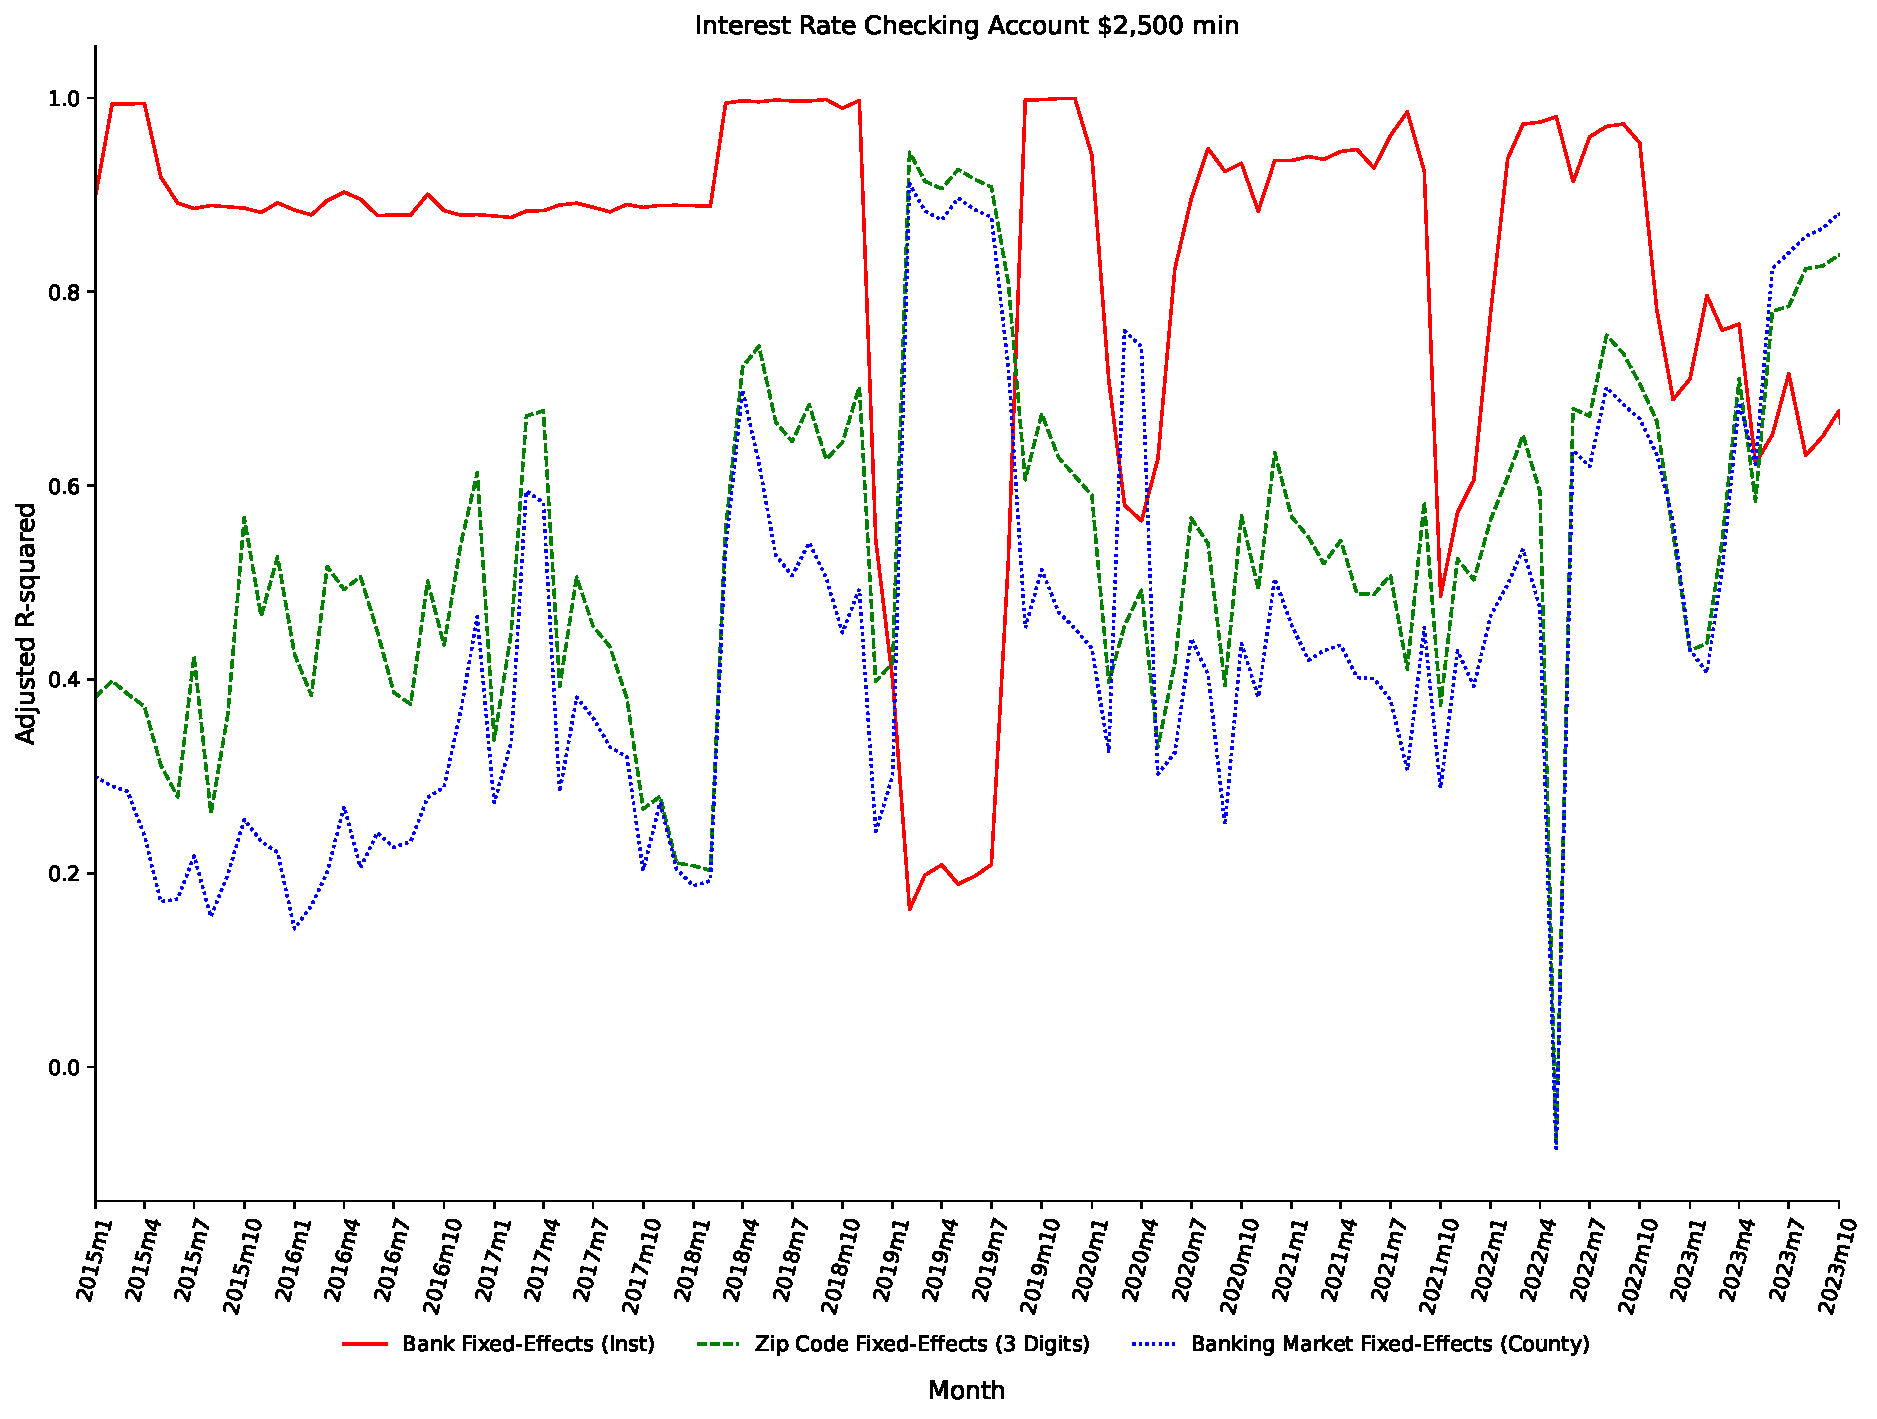
\includegraphics[width=1\textwidth]{figure/multi_branch_sample_932466/3_fixed_effects_same_as_GP_wp/INTCK2_5K_adjusted_R2_Rate_3_fixed_effects.pdf} 
\end{center}
\end{frame}

\begin{frame}{SAV25K, multi-branches sample}
\begin{center}
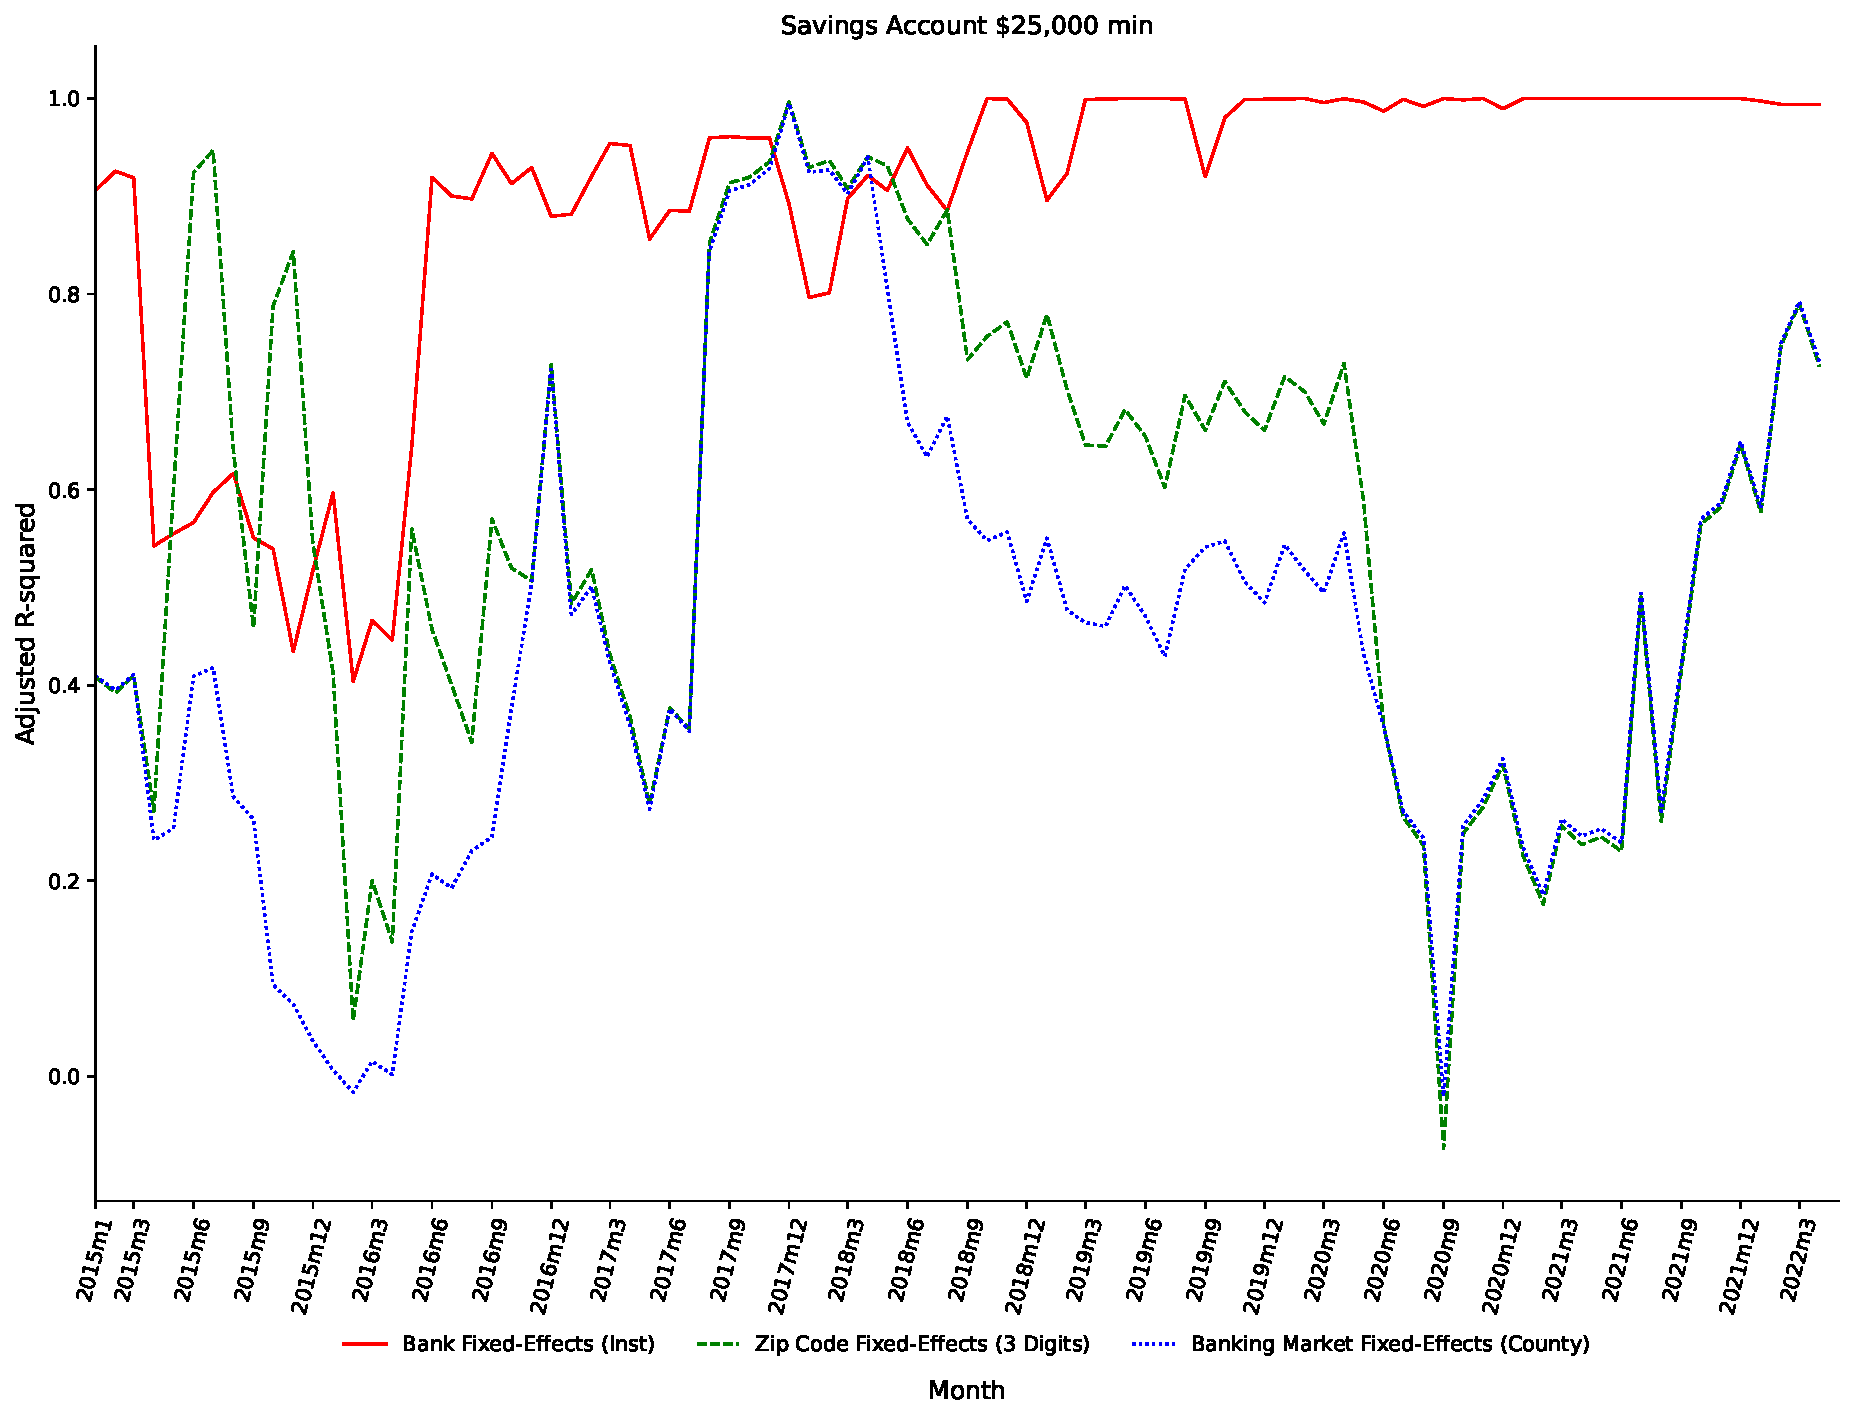
\includegraphics[width=1\textwidth]{figure/multi_branch_sample_932466/3_fixed_effects_same_as_GP_wp/SAV25K_adjusted_R2_Rate_3_fixed_effects.pdf} 
\end{center}
\end{frame}


\begin{frame}{SAV2.5K, multi-branches sample}
\begin{center}
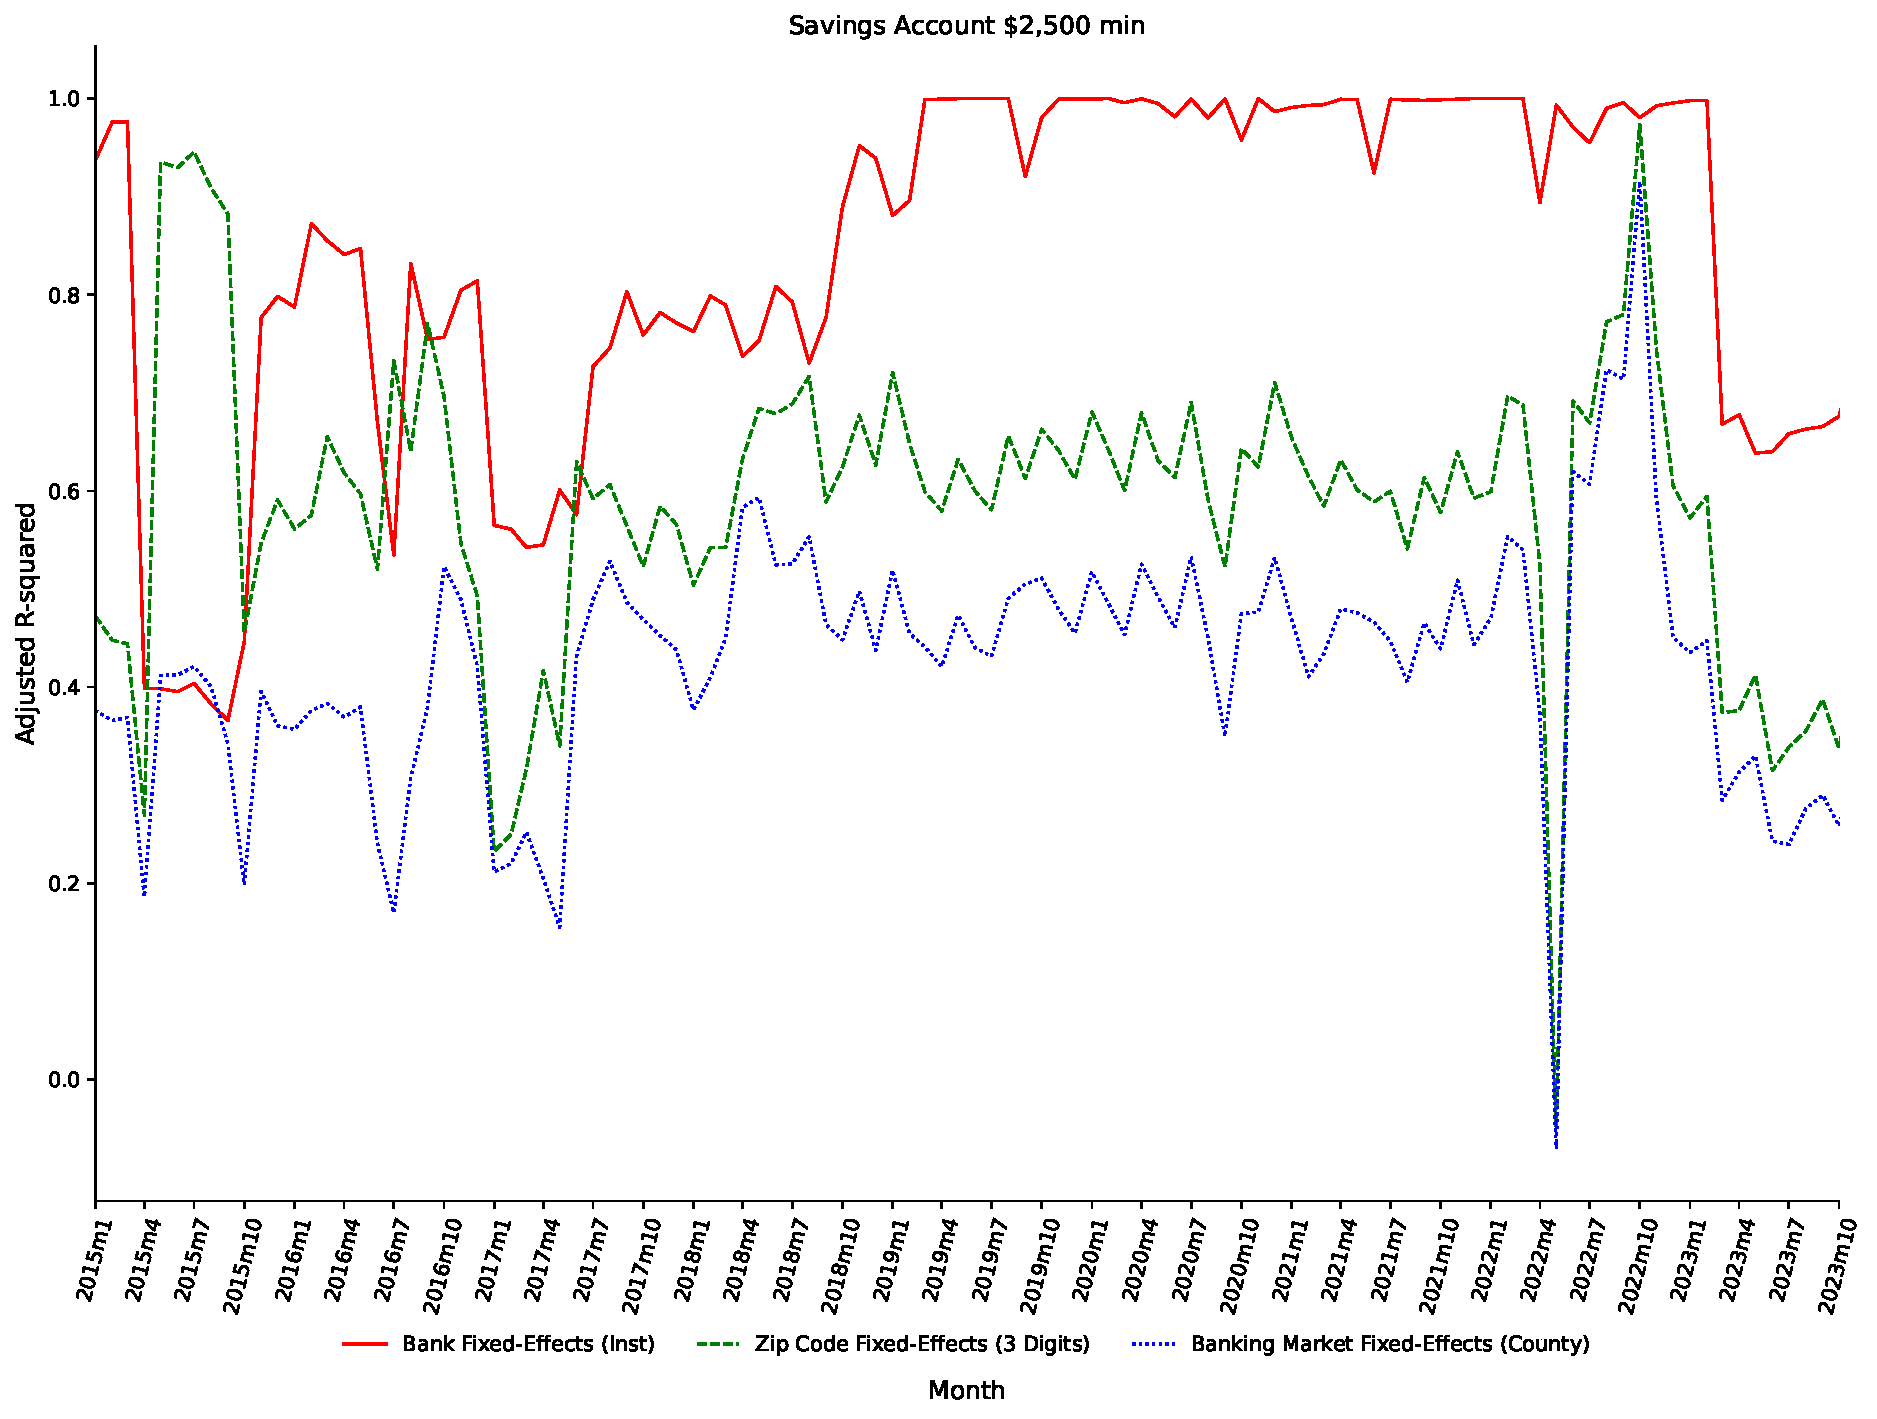
\includegraphics[width=1\textwidth]{figure/multi_branch_sample_932466/3_fixed_effects_same_as_GP_wp/SAV2_5K_adjusted_R2_Rate_3_fixed_effects.pdf} 
\end{center}
\end{frame}

\begin{frame}{Adding county fixed effects}
    \begin{itemize} 
        \item The averages across months products, for county and 3-digits fixed effects, are close.
        \begin{itemize}
            \item (multi-branches) r2\_zip3: 0.5403, r2\_county: 0.4219
            \item (all sample) r2\_zip3: 0.4409, r2\_county: 0.4225
        \end{itemize}
     \item In line charts, the $adj.R^2$ from regressions on county fixed effects and 3-digit fixed effects are relatively close and exhibit similar movements.
    \end{itemize}
\end{frame}


\begin{frame}{Adding county fixed effects}

Why county might be reasonable? The first 3 digits of a zip code and a county are not the same.

\vspace{1em}

\begin{itemize}
    \item Taking the reg data of multi-branch sample, product 12MCD10K, as an example, calculate:
    \begin{itemize}
        \item The \# of unique zip\_3digit values within each county.
        \item The \# of unique counties within each zip\_3digit.
    \end{itemize}
    \item If either of these variables $\neq$ 1, the observation count is 163,344, out of a total of 265,923 observations.
\end{itemize}

\begin{table}[]
        \centering
        \footnotesize
        \begin{tabular}{lcc}
            \hline
            & zip\_3digit\_count\_in\_county & county\_count\_in\_zip\_3digit \\
            \hline
            mean & 2.1858 & 1.5400 \\
            std & 1.7953 & 0.9514 \\
            \hline
        \end{tabular}
    \end{table}
\end{frame}



\section{Unbalanced obs. across categories of the fixed effect}

\begin{frame}
    \vfill
    \centering
    {\usebeamercolor[fg]{structure}Unbalanced obs. across categories of the fixed effect}
    \vfill
\end{frame}


\begin{frame}{Unbalanced obs. across categories of the fixed effect}
    \begin{itemize}
        \item Remember that, INTCK2.5K shows unusual periods (Dec 2018 – Aug 2019), \\
where $adj.R^2$ for fixed effects, bank $<$$<$ 3 digits zip code.
\item However, within each bank, pricing is indeed unified. So why is the overall $adj.R^2$ low in the regression?
\item The reason is that, when applying fixed effects, one needs to \textbf{consider the balance of observations across categories.}
    \end{itemize}
\end{frame}

\begin{frame}{Unbalanced obs. across categories of the fixed effect}

\textit{INTCK2.5K, Mar 2019, multi-branches}

\vspace{1em}

\small
\begin{table}[]
	\centering
	\begin{tabular}{ccccc}
		\hline
		            & \multicolumn{2}{c}{\textbf{With Wells Fargo}}    & \multicolumn{2}{c}{\textbf{No Wells Fargo}}    \\
		            & Bank FE            & 3 Zip Code FE      & Bank FE           & 3 Zip Code FE     \\ \hline
		Obs.        & 2732               & 2732               & 2488              & 2488              \\
		$R^{2}$     & 0.204              & 0.926              & 0.997             & 0.641             \\
		$adj.R^{2}$ & 0.198              & 0.914              & 0.997             & 0.580             \\ \hline
	\end{tabular}
\end{table}


\end{frame}


\begin{frame}{Unbalanced obs. across categories of the fixed effect}
\small
Take Mar 2019 of INTCK2.5K as an example, 

\begin{enumerate}
    \item Notice that the total variance for the rate is very small—almost all values are 0.01.
    \item The bank fixed effect generates several dummy variables (categorical variables). However, the number of observations within each category is highly unbalanced—Wells Fargo has 244 out of 2,732 observations, which is disproportionately high.
    \item As a result, for the rate 0.01, since Wells Fargo has the largest number of observations, this dummy variable dominates the regression results. Other banks are treated as noise, even though pricing within each bank is unified at 0.01.
\end{enumerate}

\end{frame}


\begin{frame}{Unbalanced obs. across categories of the fixed effect}
\small
\begin{itemize}
    \item In other words, because Wells Fargo has too many observations and the rate 0.01 has little variance, Wells Fargo dominates the model. Consequently, even though other banks (e.g., BoA, U.S. Bank, etc.) have the same pricing at 0.01, they are still considered noise, which lowers the $adj.R^2$ .
    \item As for zip codes, the numbers of obs within each unique 3 digits zip code is relatively balanced, resulting in a higher $adj.R^{2}$  compared to the bank fixed effect (when Wells Fargo is included in the sample).
\end{itemize}
    
\end{frame}


\section{Relation between "primarycompany" and "inst\_name" for big 4 primary companies}


\begin{frame}
    \vfill
    \centering
    {\usebeamercolor[fg]{structure}Relation between "primarycompany" and "inst\_name" for big 4 primary companies}
    \vfill
\end{frame}


\begin{frame}{Bank of America}
\begin{center}
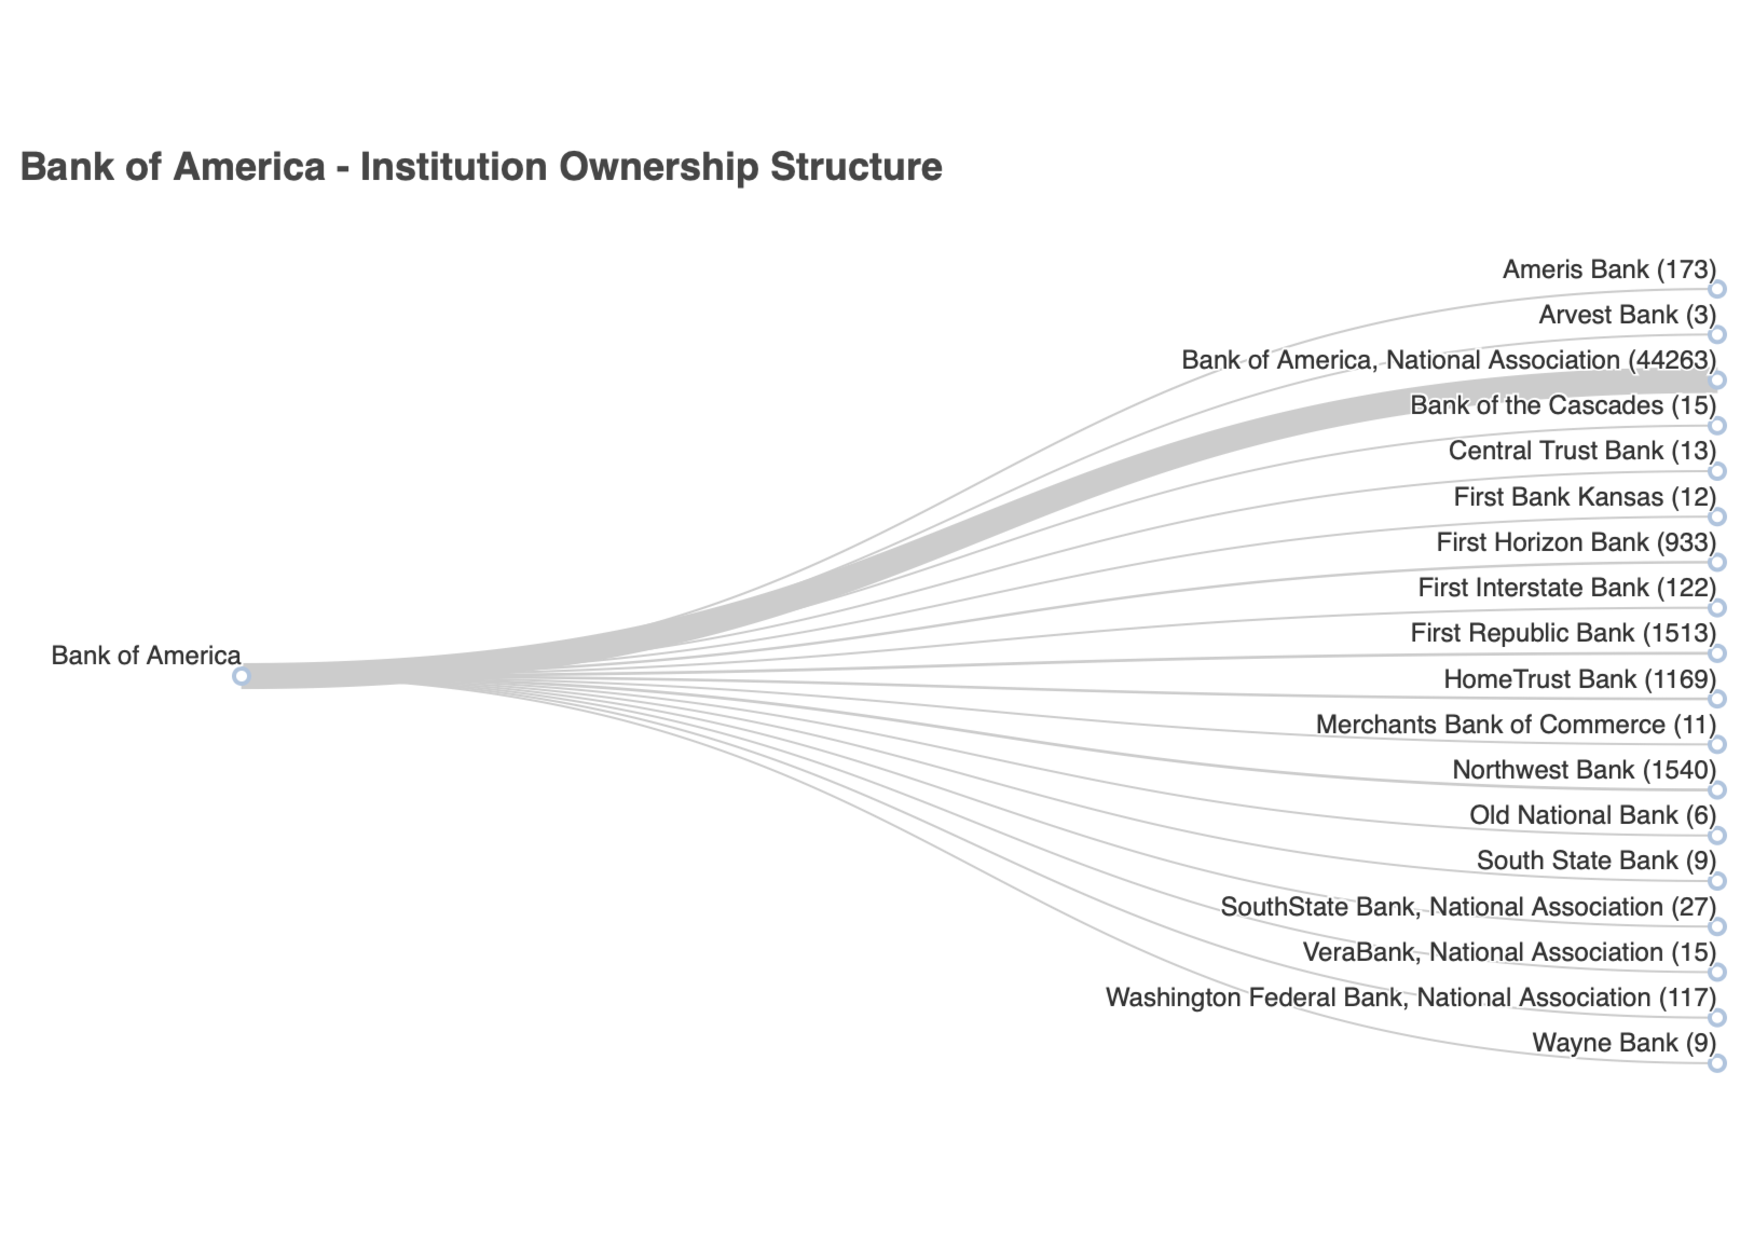
\includegraphics[width=1\textwidth]{figure/institution_ownership/Bank of America_ownership_tree.pdf} 
\end{center}
\end{frame}

\begin{frame}{Chase}
\begin{center}
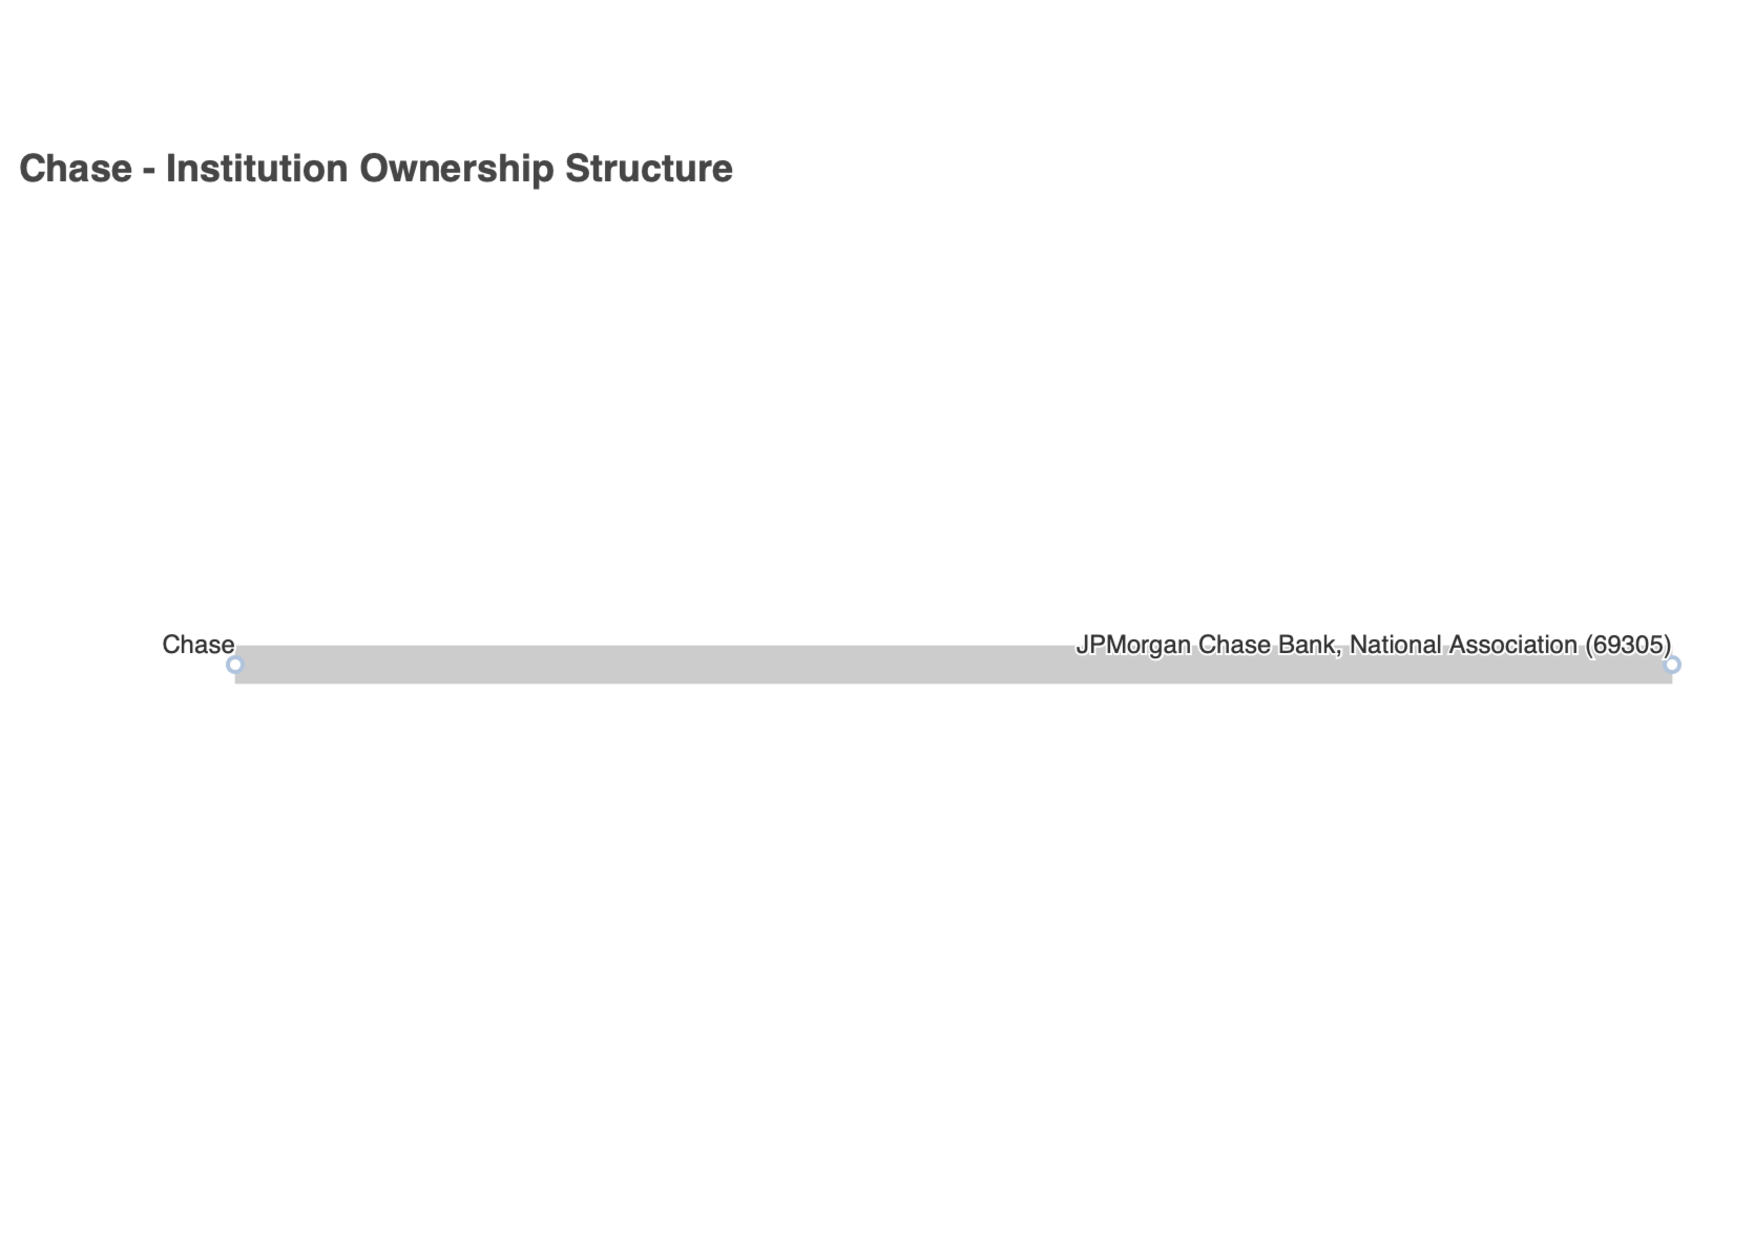
\includegraphics[width=1\textwidth]{figure/institution_ownership/Chase_ownership_tree.pdf} 
\end{center}
\end{frame}


\begin{frame}{Citibank}
\begin{center}
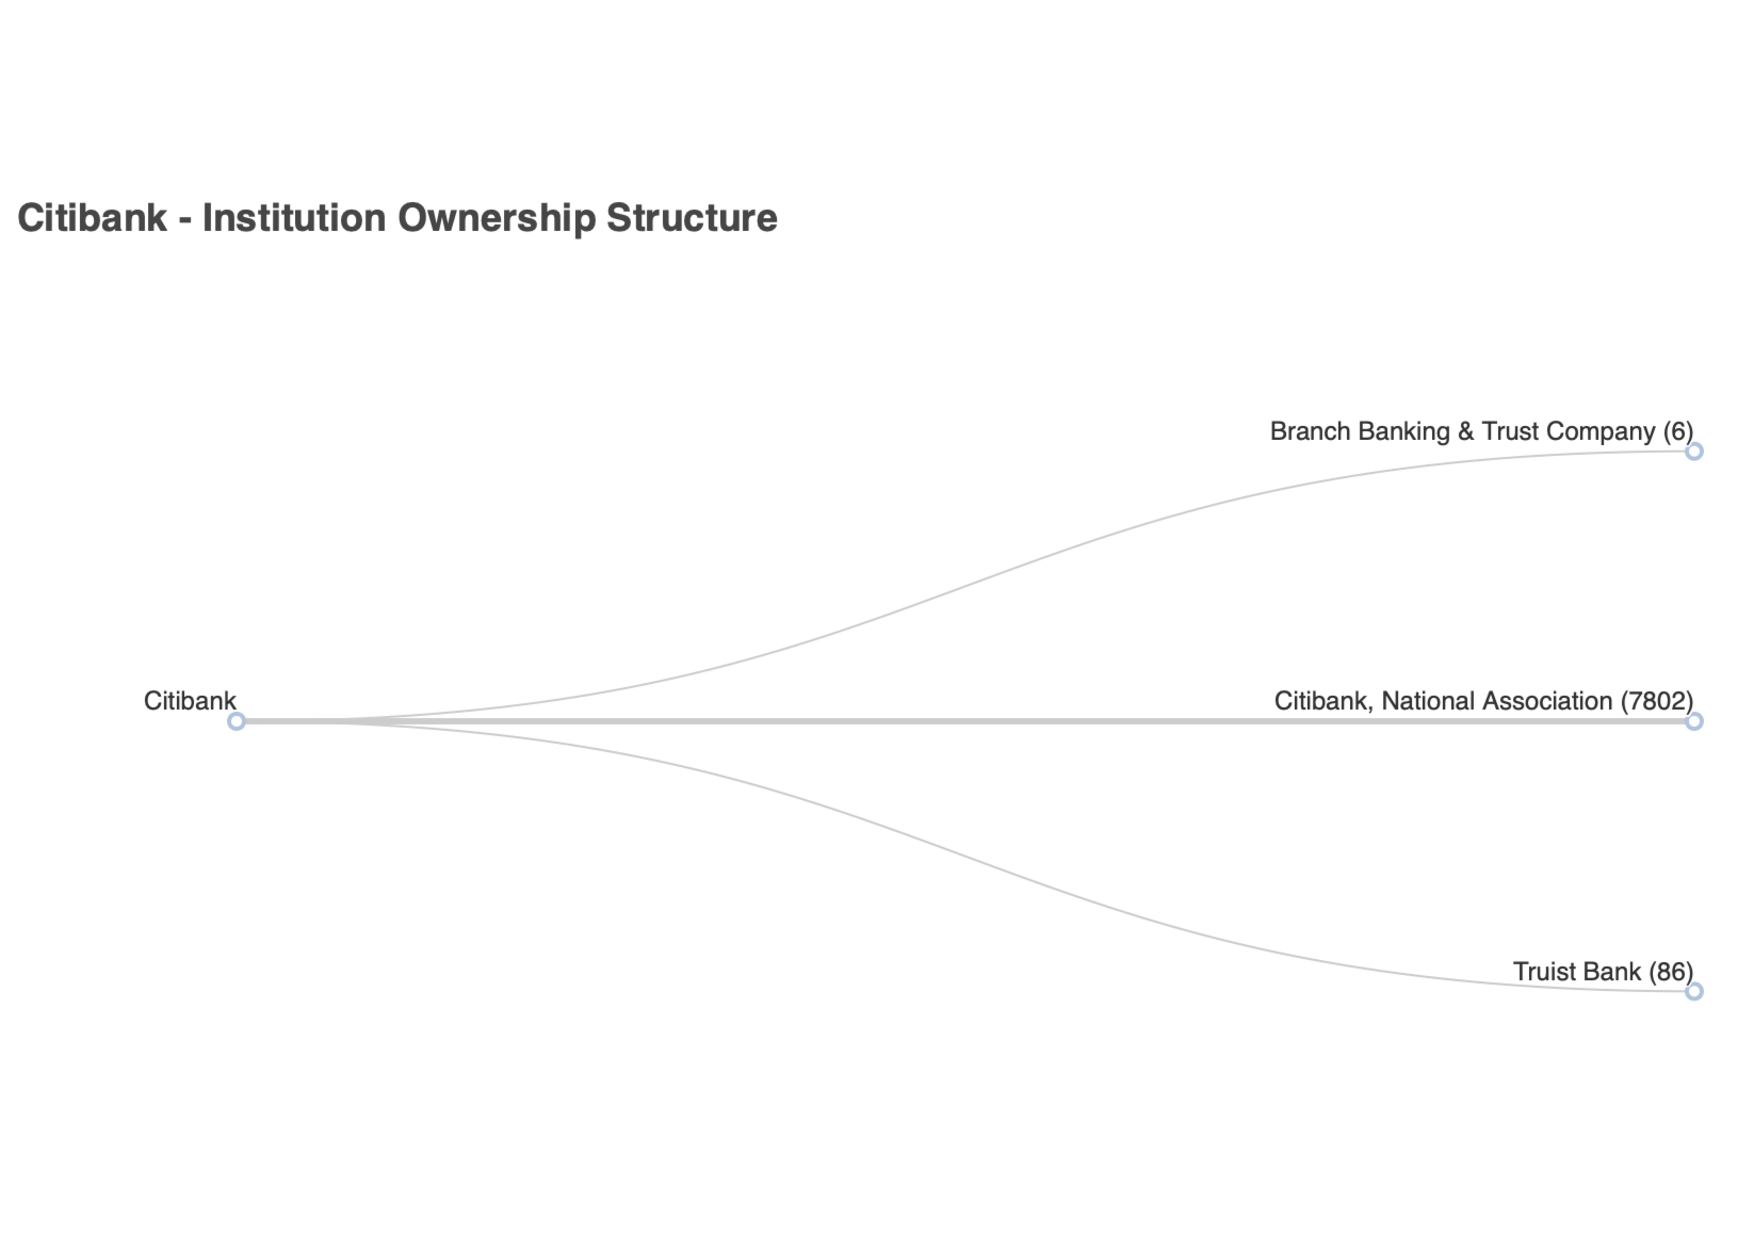
\includegraphics[width=1\textwidth]{figure/institution_ownership/Citibank_ownership_tree.pdf} 
\end{center}
\end{frame}


\begin{frame}{Wells Fargo}
\begin{center}
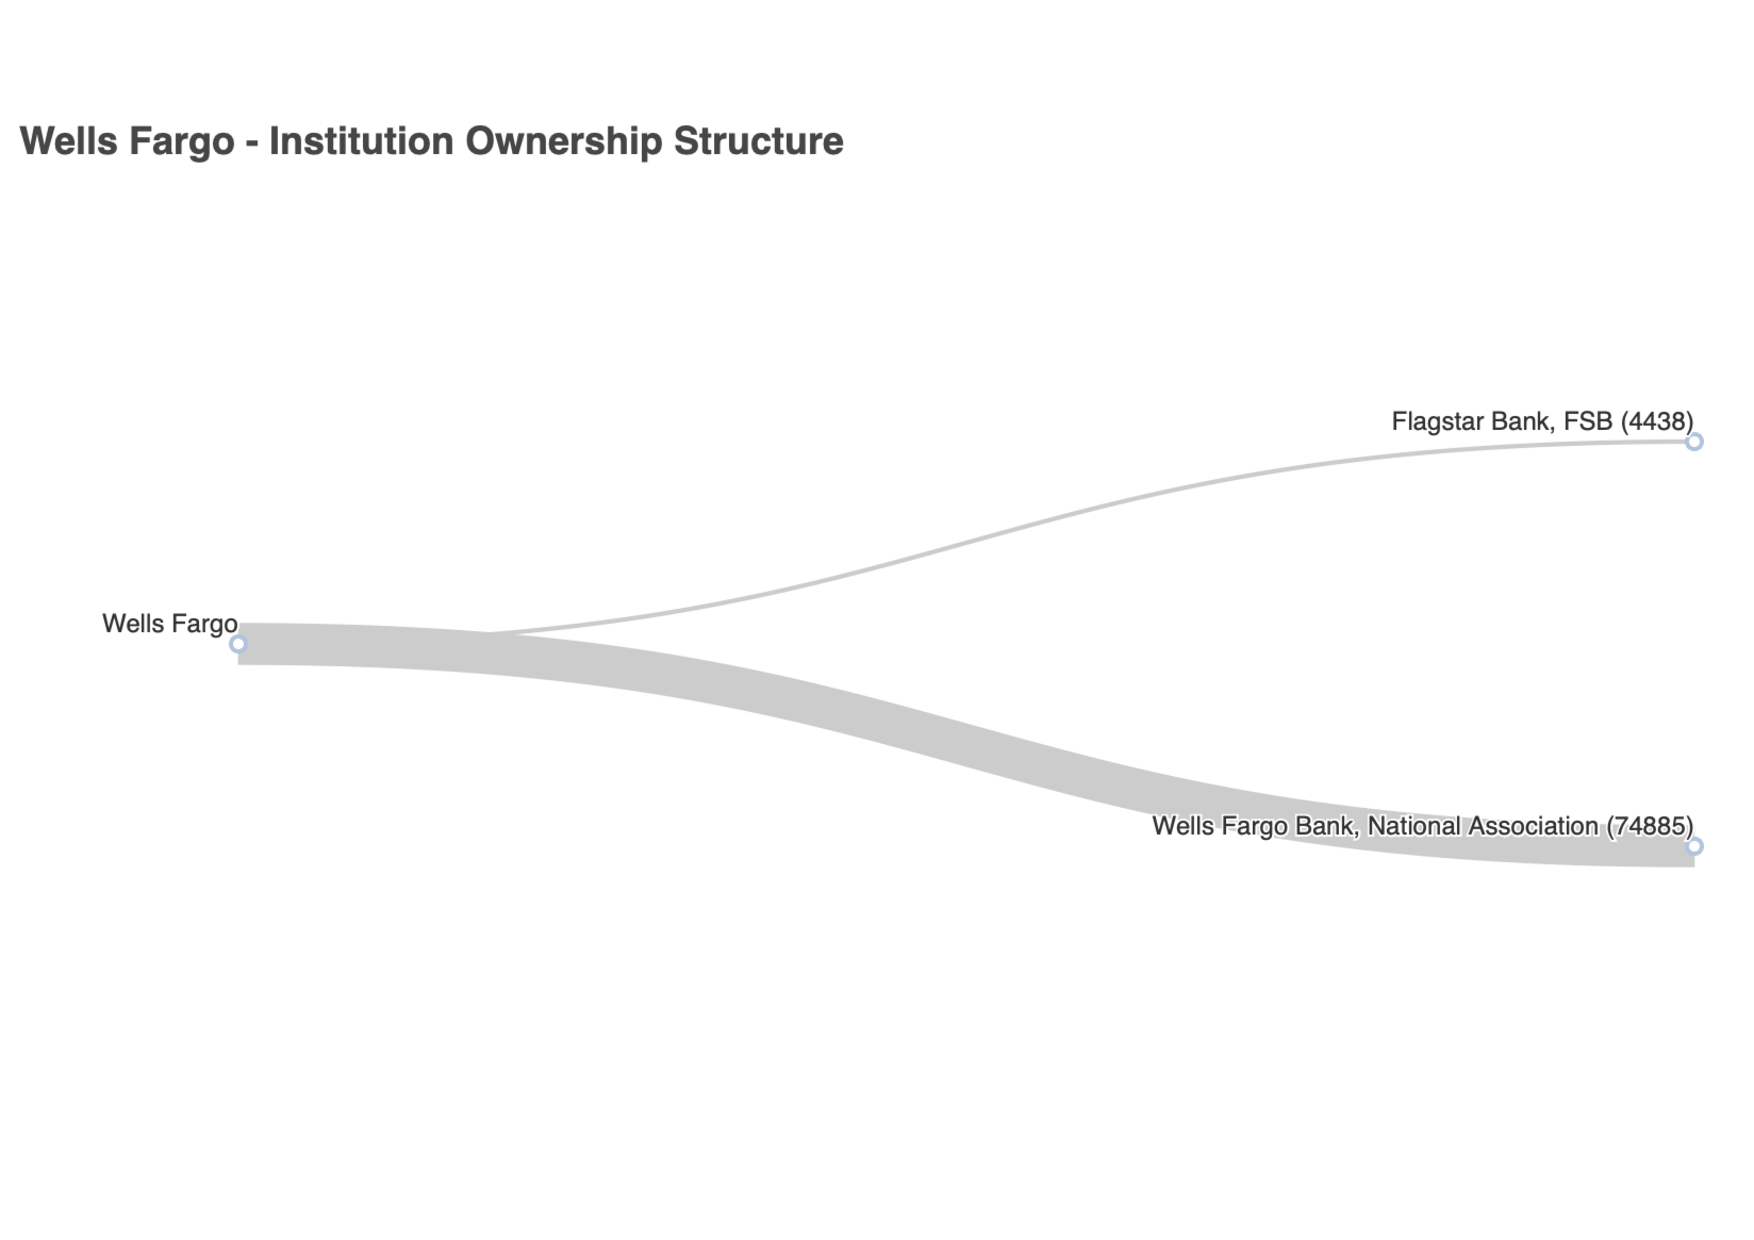
\includegraphics[width=1\textwidth]{figure/institution_ownership/Wells Fargo_ownership_tree.pdf} 
\end{center}
\end{frame}




\begin{frame}{Relation between "primarycompany" and "inst\_name" for big 4 primary companies}

\begin{itemize}
    \item The one that truly belongs to the primary company is the entity that ends with “National Association”
    \begin{itemize}
        \item Bank of America $\leftarrow$ Bank of America, National Association
\item Chase $\leftarrow$ JPMorgan Chase Bank, National Association
\item Citibank $\leftarrow$ Citibank, National Association
\item Wells Fargo $\leftarrow$ Wells Fargo Bank, National Association
    \end{itemize}
    \item Other institutions have acquired branches from these primary companies. Detailed branch data can be found in {\footnotesize \texttt{bank\_institution\_ownership\_NotNationalAssociation\_detail.xlsx}}
    \item When conducting analysis, filter out samples where inst\_nm does not belong to the primary company due to early-year acquisitions?
\end{itemize}

\end{frame}


\end{document}